% Reading order of the whole book. Moving a chapter means moving its \include
% line here; file names never change.
%
% Layout and styling come from the Legrand Orange Book template
% (LegrandOrangeBook.cls, CC BY-NC-SA 4.0, https://www.LaTeXTemplates.com).
% For the website, web/latexml/LegrandOrangeBook.cls.ltxml stands in for it.
\documentclass[
  11pt,
  fleqn,     % left-align equations, as in the template
  a4paper,
  oneside,   % no blank pages before chapters; remove for a printed (two-sided) book
]{LegrandOrangeBook}
% Packages and settings on top of LegrandOrangeBook.cls, shared by every book
% built from these chapters (main.tex, and later per-part books such as
% probability-book.tex). The class already loads amsmath/amssymb/amsthm, tikz,
% xcolor, graphicx, geometry, hyperref and biblatex. Notation lives in macros.tex.

\graphicspath{{figures/}} % e.g. 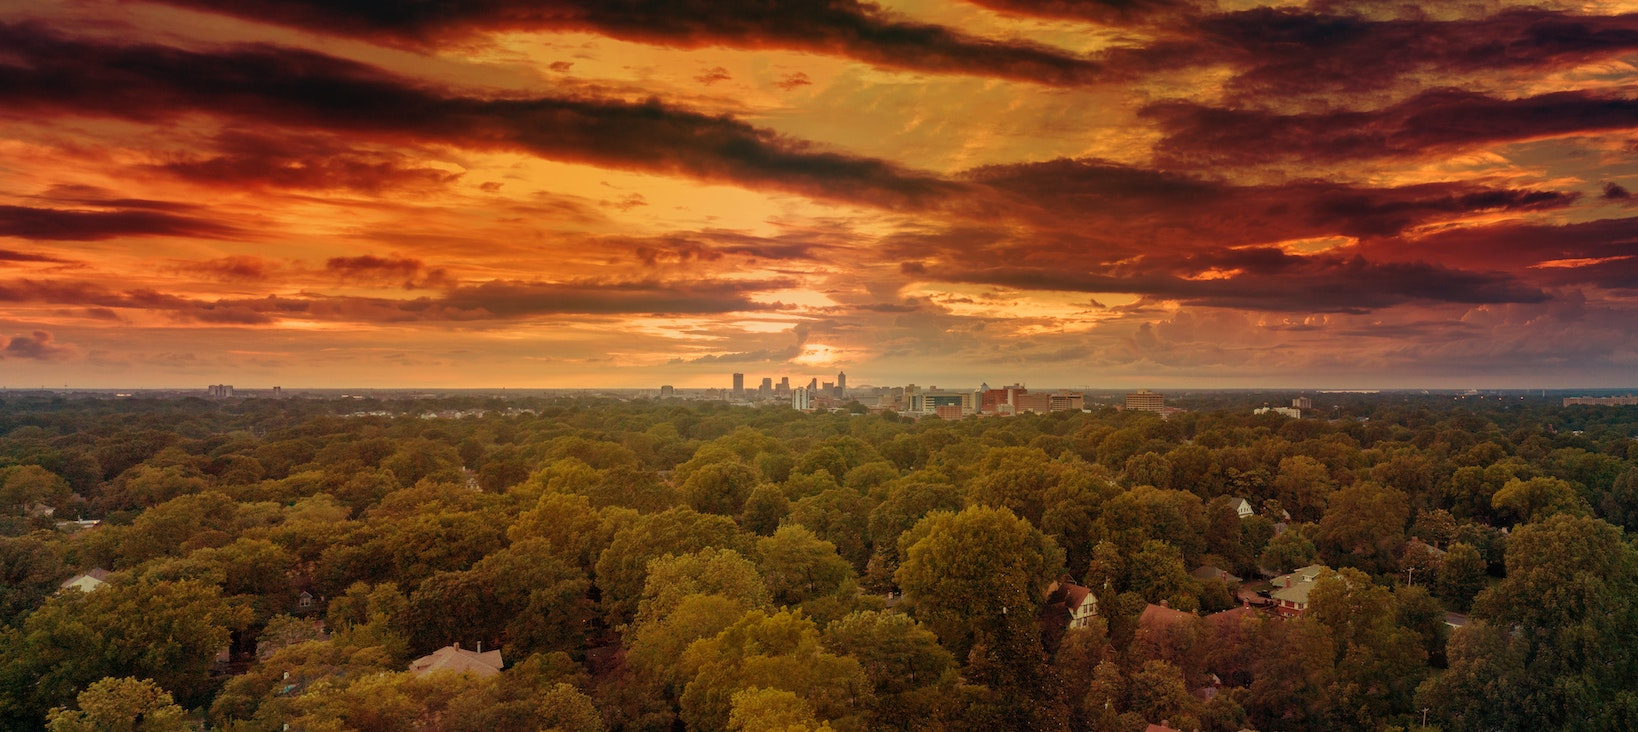
\includegraphics{template/orange1.jpg}

\usetikzlibrary{calc,decorations.pathreplacing}

\usepackage{listings}
\lstset{basicstyle=\ttfamily\small, columns=fullflexible, keepspaces=true,
        showstringspaces=false}

% Shared notation and environments. Every chapter may use these; nothing
% chapter-specific belongs here.

%--- Theorem-like environments (numbered per chapter) ---
\theoremstyle{plain}
\newtheorem{theorem}{Theorem}[chapter]
\newtheorem{proposition}[theorem]{Proposition}
\newtheorem{lemma}[theorem]{Lemma}

\theoremstyle{definition}
\newtheorem{definition}[theorem]{Definition}
\newtheorem{example}[theorem]{Example}

\theoremstyle{remark}
\newtheorem*{remark}{Remark}

%--- Chapter front matter ---
% What a chapter assumes, so a reader landing on it (e.g. on the website)
% knows what to read first. Use once, straight after \chapter and \label.
\newcommand{\assumes}[1]{%
  \par\noindent\textbf{Assumes:} #1\par\medskip}


% While writing, uncomment to rebuild only the chapter(s) you are editing
% (or use `make chapter CH=...`):
% \includeonly{chapters/probability-statistics/basic-probability}

\title{Carlo's Little Mathbook}
\author{Carlo du Toit}
\date{}

\hypersetup{
  pdftitle={Carlo's Little Mathbook},
  pdfauthor={Carlo du Toit},
  pdfsubject={Mathematics},
}

\addbibresource{refs.bib}

\definecolor{ocre}{RGB}{243, 102, 25} % highlight colour used throughout

% Default chapter heading image and spacing (overridden per part below)
\chapterimage{template/orange1.jpg}
\chapterspaceabove{6.5cm}
\chapterspacebelow{6.75cm}

\begin{document}

%----------------------------------------------------------------------------------------
%	TITLE AND COPYRIGHT PAGES
%----------------------------------------------------------------------------------------
\titlepage
  {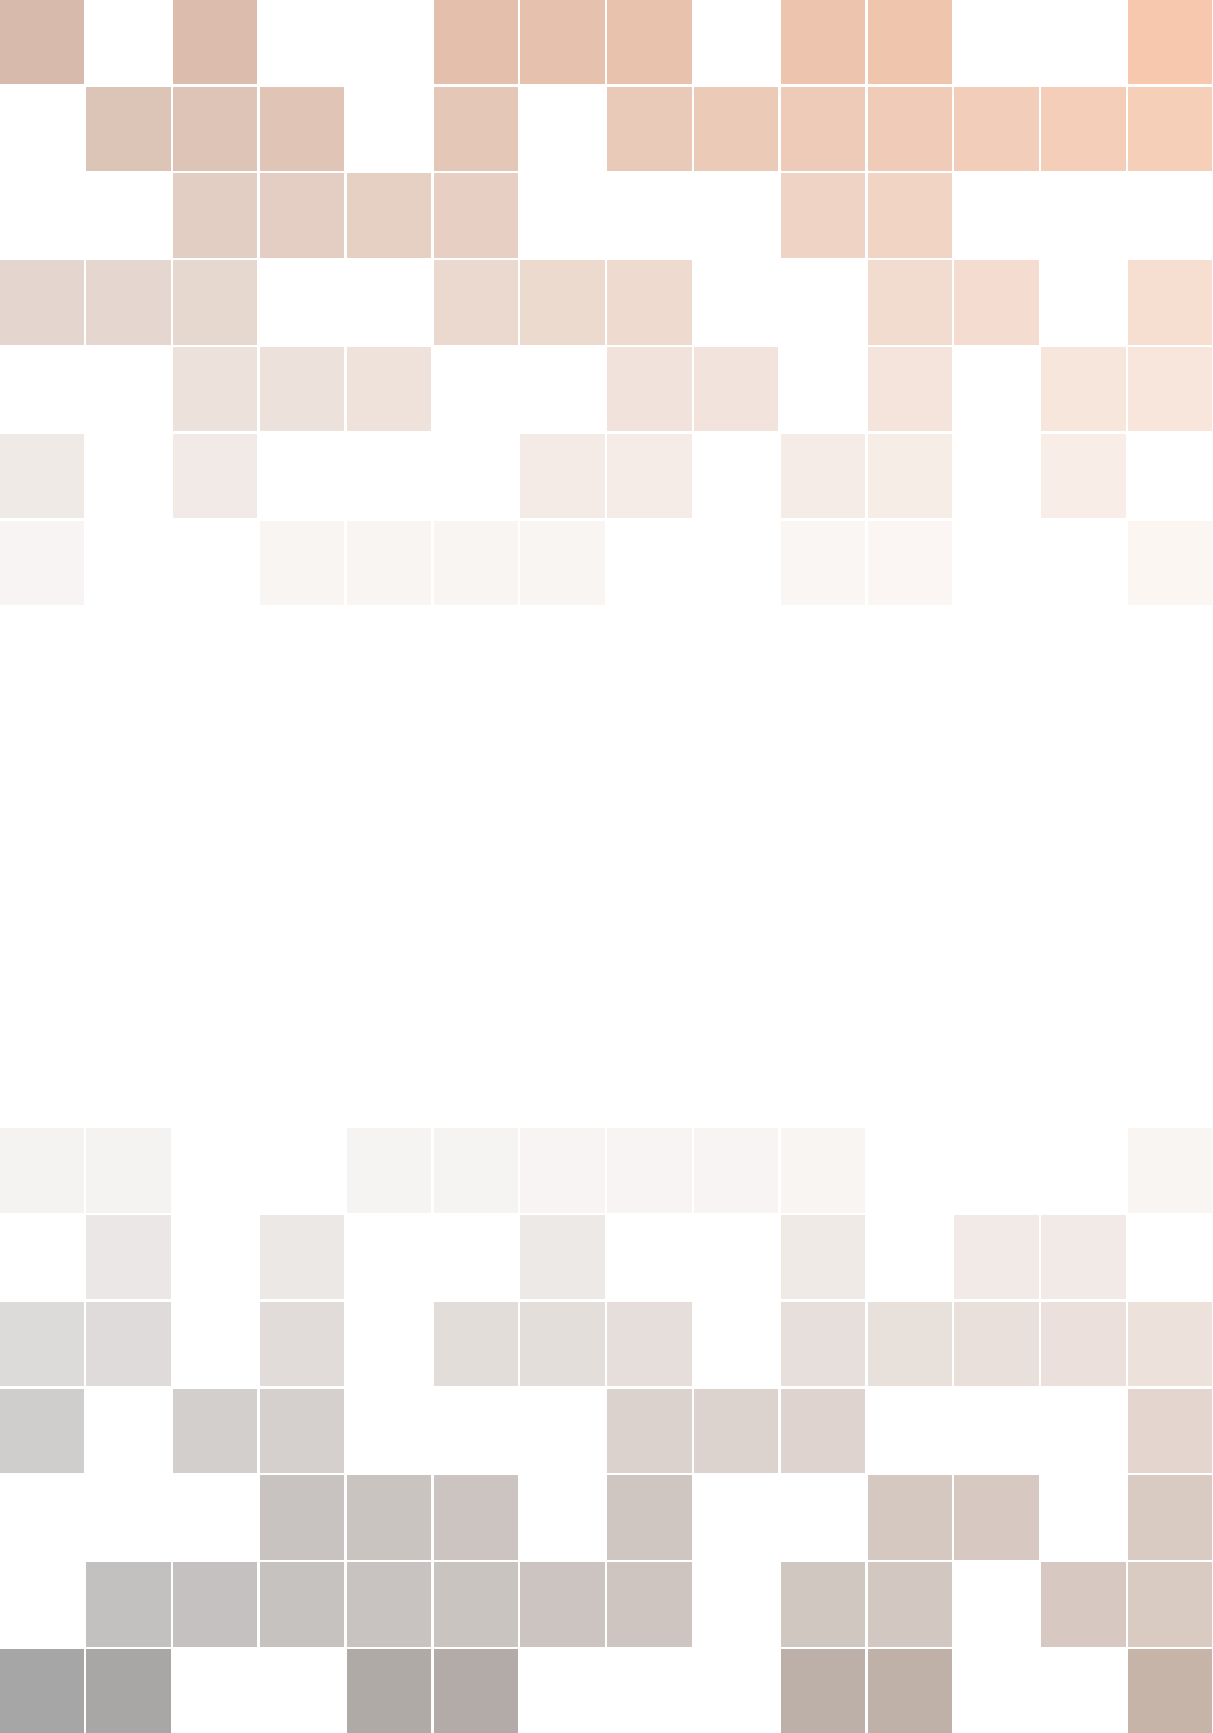
\includegraphics[width=\paperwidth]{template/background.pdf}}
  {%
    \centering\sffamily
    {\Huge\bfseries Carlo's Little Mathbook\par}
    \vspace{24pt}
    {\huge\bfseries Carlo du Toit\par}
  }

\printonly{%
\thispagestyle{empty}
~\vfill
\noindent Copyright \copyright\ 2026 Carlo du Toit\\
\noindent \textit{Typeset with the
\href{https://www.latextemplates.com/template/legrand-orange-book}{Legrand Orange Book}
template by Mathias Legrand and Vel, licensed under CC BY-NC-SA 4.0.}
}

\pagestyle{empty}
\tableofcontents
\pagestyle{fancy}
\cleardoublepage

%=========================================================
\part{Physics}\label{phys}
%=========================================================
\chapterimage{template/orange2.jpg}
\chapter{Special Relativity: Time Dilation}
\label{phys:time-dilation}

\assumes{Pythagoras' theorem; distance $=$ speed $\times$ time; the two postulates of special relativity (stated in the remark at the end).}

\begin{center}
\begin{tikzpicture}[scale=1.3]
    % Coordinates
    \coordinate (A) at (-2,0);   % base left
    \coordinate (B) at (2,0);    % base right
    \coordinate (M) at (0,0);    % base midpoint
    \coordinate (T) at (0,2.6);  % apex

    % Triangle sides (path of light on the moving ship, as seen from Earth)
    \draw[thick] (A) -- (T) -- (B);
    \draw[thick] (A) -- (B);

    % Dashed height (path of light as seen on the ship)
    \draw[dashed, thick, ->] (M) -- (T);

    % Labels for the slanted sides
    \node at (-1.15,1.5) {$L$};
    \node at (1.15,1.5) {$L$};

    % Label for height
    \node at (0.35,1.3) {$D$};

    % Tick mark showing midpoint of base
    \draw (0,-0.08) -- (0,0.08);

    % Labels for base segments
    \node at (-1,-0.3) {$S$};
    \node at (1,-0.3) {$S$};
\end{tikzpicture}
\end{center}

\noindent
\textbf{Setup:}
\begin{align*}
2D &= ct       &&\therefore D = \frac{ct}{2}     &&\text{(light's path, observer on ship)}\\
2S &= v t_0    &&\therefore S = \frac{v t_0}{2}  &&\text{(ship's speed, observer on Earth)}\\
2L &= c t_0    &&\therefore L = \frac{c t_0}{2}  &&\text{(light's path, observer on Earth)}
\end{align*}

\noindent
\textbf{Pythagorean relation:}
\[
L^2 = D^2 + S^2
\]

\noindent
\textbf{Substituting:}
\begin{align*}
\left(\frac{c t_0}{2}\right)^2 &= \left(\frac{ct}{2}\right)^2 + \left(\frac{v t_0}{2}\right)^2 \\[6pt]
\frac{c^2 t_0^2}{4} &= \frac{c^2 t^2}{4} + \frac{v^2 t_0^2}{4} \\[6pt]
\therefore\; c^2 t_0^2 &= c^2 t^2 + v^2 t_0^2 \\[6pt]
c^2 t_0^2 - v^2 t_0^2 &= c^2 t^2 \\[6pt]
\frac{c^2 t_0^2 - v^2 t_0^2}{c^2} &= t^2 \\[6pt]
t_0^2 \left(1 - \frac{v^2}{c^2}\right) &= t^2 \\[6pt]
\sqrt{t_0^2} &= \sqrt{\dfrac{t^2}{1 - \dfrac{v^2}{c^2}}} \\[6pt]
\therefore\; t_0 &= \frac{t}{\sqrt{1 - \dfrac{v^2}{c^2}}}
\end{align*}
\begin{center}
\boxed{\therefore\; t_0 = \frac{t}{\sqrt{1 - \dfrac{v^2}{c^2}}}}
\end{center}

\bigskip
\noindent\textbf{Remark.} The factor $1/\sqrt{1-v^2/c^2}$ that shows up here is important enough to have its own symbol, $\gamma$, called the \emph{Lorentz factor} -- named after Hendrik Lorentz, who worked out very similar mathematics years before Einstein published special relativity in 1905, originally to explain the null result of the Michelson--Morley experiment. It's worth looking at the two extremes: for everyday speeds ($v \ll c$), $\gamma \approx 1$ and $t_0 \approx t$, which is exactly why nobody notices time dilation in ordinary life; but as $v \to c$, $\gamma \to \infty$, so a clock moving at (nearly) the speed of light appears, to an outside observer, to almost stop. What makes this especially striking is how little was assumed to derive it: just that the laws of physics look the same in every inertial frame, and that the speed of light $c$ is the same for \emph{every} observer, no matter how fast the light source is moving -- two simple postulates producing a deeply counter-intuitive conclusion.

\chapter{Centripetal Acceleration}
\label{phys:centripetal-acceleration}

\assumes{Similar triangles; velocity as a vector; acceleration as the rate of change of velocity; limits.}

\begin{center}
\begin{minipage}{0.5\textwidth}
\centering
\begin{tikzpicture}[scale=1.1]
    \def\R{2}
    \coordinate (O) at (0,0);
    \def\aOne{100}
    \def\aTwo{72}
    \coordinate (P1) at (\aOne:\R);
    \coordinate (P2) at (\aTwo:\R);

    \draw[thick] (O) circle (\R);
    \fill (O) circle (1.3pt);

    \draw[thick] (O) -- (P1) node[midway, above left] {$r$};
    \draw[thick] (O) -- (P2) node[midway, above right] {$r$};

    % tangent velocity vectors (perpendicular to radius, direction of travel)
    \draw[thick,->] (P1) -- ($(P1)+(\aOne+90:1.3)$) node[above] {$v_1$};
    \draw[thick,->] (P2) -- ($(P2)+(\aTwo+90:1.3)$) node[above right] {$v_2$};
\end{tikzpicture}
\end{minipage}%
\begin{minipage}{0.42\textwidth}
\centering
% --- Triangle A: angle relation theta ---
\begin{tikzpicture}[scale=0.85]
    \coordinate (Top) at (0,2);
    \coordinate (Left) at (-1.3,0.6);
    \coordinate (Right) at (1.3,0.6);
    \coordinate (Bottom) at (0,-0.8);
    \draw (Left) -- (Top) -- (Right);
    \draw (Left) -- (Bottom) -- (Right);
    \node at (0,1.55) {$\theta$};
    \node at (0,-0.35) {$\theta$};
    \draw (Left)++(0.18,0.05) -- ++(0.15,0.18) -- ++(0.18,-0.13);
    \draw (Right)++(-0.18,0.05) -- ++(-0.15,0.18) -- ++(-0.18,-0.13);
\end{tikzpicture}

\vspace{6pt}
% --- Triangle B: Delta v triangle ---
\begin{tikzpicture}[scale=0.85]
    \coordinate (Apex) at (0,0);
    \coordinate (TopLeft) at (-1.3,1.6);
    \coordinate (TopRight) at (1.3,1.6);
    \draw[thick] (Apex) -- (TopLeft);
    \draw[thick] (Apex) -- (TopRight);
    \draw[thick,->] (TopRight) -- (TopLeft);
    \node at (0,1.9) {$\Delta v$};
    \node at (-1.2,0.8) {$v_2$};
    \node at (1.2,0.8) {$v_1$};
\end{tikzpicture}

\vspace{6pt}
% --- Triangle C: Delta s triangle (same orientation as Delta v triangle above) ---
\begin{tikzpicture}[scale=0.85]
    \coordinate (Apex) at (0,0);
    \coordinate (TopLeft) at (-1.3,1.6);
    \coordinate (TopRight) at (1.3,1.6);
    \draw[thick] (Apex) -- (TopLeft) -- (TopRight) -- cycle;
    \node at (-1.2,0.8) {$r$};
    \node at (1.2,0.8) {$r$};
    \node at (0,1.9) {$\Delta s$};
\end{tikzpicture}
\end{minipage}
\end{center}

\noindent
Given the above, we can say:
\begin{equation}
\frac{\Delta v}{v_1} = \frac{\Delta s}{r}
\qquad
\therefore\; \Delta v = \frac{\Delta s \, v_1}{r}
\label{phys:eq:delta-v}
\end{equation}

\noindent
\textbf{Average acceleration:}
\[
a_{avg} = \frac{\Delta v}{\Delta t}
\]

\noindent
Substitute \eqref{phys:eq:delta-v} into the above:
\[
a_{avg} = \frac{\Delta s \, v_1}{\Delta t \, r}
\]

\[
a_{inst} = \lim_{\Delta t \to 0} \frac{\Delta s \, v_1}{\Delta t \, r}
\]

\noindent
We know that $\displaystyle\lim_{\Delta t \to 0} \frac{\Delta s}{\Delta t} = v = v_1$, therefore:
\[
a_{inst} = \frac{v_1 \cdot v_1}{r} = \frac{v_1^2}{r} = \frac{v^2}{r}
\]

\begin{center}
\boxed{\,a = \dfrac{v^2}{r}\,}
\end{center}

\bigskip
\noindent\textbf{Remark.} The derivation above only gives the \emph{magnitude} of the acceleration, but the direction is worth pointing out too: as $\Delta t \to 0$, the vector $\Delta \vec{v}$ rotates to point directly toward the centre $O$ of the circle -- which is exactly why this is called \emph{centripetal} acceleration, from the Latin \textit{centrum petere}, "to seek the centre." This resolves a common source of confusion: in uniform circular motion the \emph{speed} $v$ never changes, yet the object is still accelerating, because acceleration measures the rate of change of the \emph{velocity vector} -- and here it's the \emph{direction} of that vector that is constantly changing, not its length. Historically, this result predates Newton's \textit{Principia} (1687): Christiaan Huygens worked out the same formula around 1659, making it one of the earliest quantitative results in dynamics.


%=========================================================
\part{Probability and Statistics}\label{prob}
%=========================================================
\chapterimage{template/orange3.jpg}
\chapter{Basic Probability}
\label{prob:basic-probability}

\assumes{Sums and integrals; the idea of a probability distribution over discrete or continuous outcomes.}

\section{Fundamental Rules}
\label{prob:sec:fundamental-rules}

\begin{align}
\text{Sum Rule:} && p(x) &= \sum_{y} p(x,y) \label{prob:eq:sum-rule} \\
\text{Product Rule:} && p(x,y) &= p(y\mid x)\,p(x) \label{prob:eq:product-rule}
\end{align}

\noindent
These two rules, \eqref{prob:eq:sum-rule} and \eqref{prob:eq:product-rule}, are nicely derived in Chris Bishop's book~\cite{bishop2006prml} using Fig.\ 1.10 (p.\ 13). From these two rules alone, a great many other identities can be derived, e.g.\ the joint-histogram picture below.

\begin{center}
\begin{tikzpicture}[scale=0.65]
    \draw (0,0) grid (5,3);
    \node at (-0.7,1.5) {$y_j$};
    \node at (2.5,-0.6) {$x_i$};
    \draw[decorate,decoration={brace,amplitude=6pt}] (5.2,0) -- (5.2,3) node[midway,right=10pt] {$c_i$};
    \draw[decorate,decoration={brace,amplitude=6pt,mirror}] (0,3.2) -- (5,3.2) node[midway,above=10pt] {$r_j$};
\end{tikzpicture}
\end{center}
\[
p(x_i,y_j) = \frac{n_{ij}}{N}, \qquad p(x_i) = \frac{c_i}{N}
\]

\noindent
\textbf{Conditional probability} -- from the product rule:
\[
p(y\mid x) = \frac{p(y,x)}{p(x)}
\]

\noindent
Using the rule of symmetry that $p(x,y) = p(y,x)$, we derive the (in)famous \textbf{Bayes' theorem}. Since
\[
p(x\mid y) = \frac{p(x,y)}{p(y)}
\qquad \text{also} \qquad
p(y\mid x) = \frac{p(y,x)}{p(x)},
\]
then $p(x\mid y)\,p(y) = p(y\mid x)\,p(x)$, so:
\begin{equation}
\boxed{\,p(x\mid y) = \dfrac{p(y\mid x)\,p(x)}{p(y)}\,}
\label{prob:eq:bayes}
\end{equation}

\section{Total Probability, from Bayes' Theorem}
\label{prob:sec:total-probability}

\noindent
From Bayes' theorem we can derive the total probability equation. From \eqref{prob:eq:bayes}:
\[
p(x\mid y) = \frac{p(y\mid x)\,p(x)}{p(y)}
\]
If we integrate both sides of the equation with respect to $x$ we get:
\[
\int p(x\mid y)\,dx = \int \frac{p(y\mid x)\,p(x)}{p(y)}\,dx
\]
Since $p(y)$ can be seen as a constant and is not a function of $x$, we can move it outside of the integral:
\[
\int p(x\mid y)\,dx = \frac{1}{p(y)} \int p(y\mid x)\,p(x)\,dx
\]
On the left-hand side, if $y$ is fixed (constant) and we integrate with respect to $x$, the axioms of probability tell us that $\int p(x\mid y)\,dx = 1$. Therefore:
\[
1 = \frac{1}{p(y)} \int p(y\mid x)\,p(x)\,dx
\]
\begin{equation}
\boxed{\,p(y) = \int p(y\mid x)\,p(x)\,dx\,}
\label{prob:eq:total-probability}
\end{equation}

\section{Bayes Classifier -- A Speaker Recognition Example}
\label{prob:sec:bayes-classifier}

\noindent
Understanding Bayes' theorem as \emph{posterior} $\propto$ \emph{likelihood} $\times$ \emph{prior} is very well explained in an example (Bishop~\cite[p.~17]{bishop2006prml}). This example also explains independence nicely.

\medskip
\noindent
\textbf{Understanding a Bayes classifier using a speaker recognition example.} Suppose we have training data of $3$ speakers $C_1, C_2, C_3$. If we receive a sample (random) $x$ and would like to identify who has spoken, Bayes' theorem would be written as:
\[
p(C_i\mid x) = \frac{p(x\mid C_i)\,p(C_i)}{p(x)} = \frac{p(x\mid C_i)\,p(C_i)}{\sum_i p(x\mid C_i)\,p(C_i)}
\]

\noindent
This would read as: the probability of being class $C_i$ given random $x$, $\big[p(C_i\mid x)\big]$, is equal to the probability of $x$ given $C_i$ times $p(C_i)$, divided by the sum over all speakers of the probability of $x$ given $C_i$ times $p(C_i)$.

\medskip
\noindent
E.g.\ the probability that $x$ is speaker $2$ is:
\[
p(C_2\mid x) = \frac{p(x\mid C_2)\,p(C_2)}{p(x\mid C_1)p(C_1) + p(x\mid C_2)p(C_2) + p(x\mid C_3)p(C_3)}
\]

\noindent
$p(C_2)$ is called the \emph{prior} estimate, before given the observation; $p(x\mid C_2)$ is the \emph{likelihood function}; and $\displaystyle\sum_i p(x\mid C_i)p(C_i)$ is the \emph{normalising constant}.

\section{General Probability Rules}
\label{prob:sec:general-rules}

\noindent
\textbf{Chain rule:}
\begin{align*}
p(z_0,z_1,z_2) &= p(z_2\mid z_0,z_1)\,p(z_0,z_1) \\
&= p(z_2\mid z_0,z_1)\,p(z_1\mid z_0)\,p(z_0)
\end{align*}

\noindent
In general form, given vector $\vec x = \{x_1,\dots,x_K\}$:
\[
p(\vec x) = \prod_{k=1}^{K} p(x_k \mid pa_k)
\]
where $pa_k$ denotes the set of parents of $x_k$.

\medskip
\noindent
Also,
\[
p(A,B) = p(B\mid A)\,p(A) \quad \text{or} \quad p(A\mid B)\,p(B),
\]
\[
p(A,B,C) = p(A\mid B,C)\,p(B,C) \quad \text{or} \quad p(A,B\mid C)\,p(C).
\]
The chain rule can be applied again on whichever grouped term remains -- you can choose what to group together.

\medskip
\noindent
\textbf{Marginal probability} -- from Bayes,
\[
p(y\mid x) = \frac{p(x\mid y)\,p(y)}{p(x)}
\]
Summing both sides over $y \in A_y$:
\[
1 = \sum_{y\in A_y} p(y\mid x) = \frac{1}{p(x)} \sum_{y\in A_y} p(x\mid y)\,p(y)
\]
\[
\therefore\; p(x) = \sum_{y\in A_y} p(x\mid y)\,p(y)
\]
\noindent
or, using conditional probability,
\[
p(x) = \sum_{y\in A_y} p(x,y)
\qquad \text{(continuous case: } p(x) = \int_y p(x,y)\,dy \text{)}
\]

\medskip
\noindent
\textbf{Statistical independence} -- if $p(x\mid y) = p(x)$, then the conditional probability does not depend on $y$. Thus $X$ and $Y$ are statistically independent. Also,
\[
p(x,y) = p(x\mid y)\,p(y) = p(x)\,p(y)
\]

\medskip
\noindent
\textbf{Conditional independence.} $X$ and $Y$ are conditionally independent given $Z$ if
\[
p(x,y\mid z) = p(x\mid z)\,p(y\mid z)
\qquad \text{also written} \qquad
X \perp\!\!\!\perp Y \mid Z.
\]

\noindent
\textbf{To show this:} by the product rule,
\[
p(x,y\mid z) = p(y\mid x,z)\,p(x\mid z)
\]
Since $X$ and $Y$ are conditionally independent given $Z$, the term $p(y\mid x,z)$ reduces to $p(y\mid z)$, because $X$ and $Y$ are independent (given $Z$). We then get:
\[
p(x,y\mid z) = p(y\mid z)\,p(x\mid z)
\]

\section{Application: The Monty Hall Problem}
\label{prob:sec:monty-hall}

\noindent
Game show where there is a car behind $1$ of $3$ doors. On the first go you select a door, then the gameshow host selects a door that does not contain the car or your first choice. Essentially, now there are only $2$ doors left where the car can be. The question is: do you stick with your original choice, or move to the next door? The answer is very interesting, and can be shown using conditional probability.

\begin{center}
\begin{tikzpicture}[scale=1]
    \foreach \i/\lbl in {0/A,1/B,2/C} {
        \draw[thick] (1.4*\i,0) rectangle (1.4*\i+1.1,1.8);
        \node at (1.4*\i+0.55,-0.4) {Door \lbl};
    }
\end{tikzpicture}
\end{center}

\noindent
Sample space $S = \{A,B,C\}$ (Doors $A$--$C$). Now define events: the event that the car is behind door $A$ is $X_A$; similarly, $B \to X_B$, etc. So $\mathfrak{X} = \{X_A, X_B, X_C\}$, and
\[
p(X_A) = \tfrac13, \qquad p(X_B) = \tfrac13, \qquad p(X_C) = \tfrac13.
\]
Say we choose Door $A$.

\medskip
\noindent
Now define the event of the gameshow host choosing a door, $\mathfrak{Y} = \{Y_A, Y_B, Y_C\}$, where $Y_A$ is the event that he chooses door $A$ (etc.).

\medskip
\noindent
Given our first choice, we can write the following conditional probabilities: $p(Y_i \mid X_i)$ -- reading this as the probability the gameshow host chooses door $Y_i$ given the car is behind door $X_i$. Now compute the permutations
\begin{center}
\begin{tabular}{lll}
$p(Y_A\mid X_A)=0$ & $p(Y_B\mid X_A)=\tfrac12$ & $p(Y_C\mid X_A)=\tfrac12$ \\[4pt]
$p(Y_A\mid X_B)=0$ & $p(Y_B\mid X_B)=0$ & $p(Y_C\mid X_B)=1^{*}$ \\[4pt]
$p(Y_A\mid X_C)=0$ & $p(Y_B\mid X_C)=1^{*}$ & $p(Y_C\mid X_C)=0$
\end{tabular}
\end{center}
\noindent
(We chose Door $A$, and according to the rules he must not select the door we chose. $^{*}$Remember, he also cannot choose the door containing the car; therefore he will choose that door with $100\%$ certainty.)

\medskip
\noindent
Ultimately we would like to know: if the game show host chooses, say, Door $C$, should we stick with $A$ or go to $B$? To calculate this we need to compute the following equations:
\[
\text{(1)}\ \ p(X_A\mid Y_C) \qquad\qquad \text{(2)}\ \ p(X_B \mid Y_C)
\]

\medskip
\noindent
\textbf{(1) Bayes' rule + sum rule:}
\begin{align*}
p(X_A\mid Y_C) &= \frac{p(Y_C\mid X_A)\,p(X_A)}{p(Y_C)}
= \frac{p(Y_C\mid X_A)\,p(X_A)}{p(Y_C\mid X_A)p(X_A)+p(Y_C\mid X_B)p(X_B)+p(Y_C\mid X_C)p(X_C)} \\[8pt]
&= \frac{\tfrac12\times\tfrac13}{\left(\tfrac12\times\tfrac13\right)+\left(1\times\tfrac13\right)+\left(0\times\tfrac13\right)}
= \frac{\tfrac16}{\tfrac16+\tfrac13+0}
= \frac{\tfrac16}{\tfrac36}
= \tfrac16 \times \tfrac63 = \tfrac13 \approx 33\%
\end{align*}
if you stick with your original choice.

\medskip
\noindent
\textbf{(2)}
\[
p(X_B\mid Y_C) = \frac{p(Y_C\mid X_B)\,p(X_B)}{p(Y_C)}
= \frac{p(Y_C\mid X_B)\,p(X_B)}{p(Y_C\mid X_A)p(X_A)+p(Y_C\mid X_B)p(X_B)+p(Y_C\mid X_C)p(X_C)}
\]
From the previous calculation we know $p(Y_C) = \tfrac36$. Now:
\[
p(X_B\mid Y_C) = \frac{p(Y_C\mid X_B)\,p(X_B)}{\tfrac36}
= \frac{1\times\tfrac13}{\tfrac36}
= \frac{\tfrac13}{\tfrac36}
= \tfrac13\times\tfrac63 = \tfrac69 = \boxed{\tfrac23}
\approx 67\%,
\]
Therefore, it is better to change your original choice.

\medskip
\noindent
\textbf{Intuition.} Most would think that after the game show host removes one door, the odds change to $50/50$; but with him eliminating a door there is some information leaking and when calculating it it becomes apparent what this information was. He knows where the car is, and with the rules of the game, if he makes his choice, there is some valuable information that we can use from this.

\webonly{
\begin{explore}[Simulate it]
Rather than trust the algebra, play the game a hundred thousand times. This
script always picks door $A$, lets the host open a goat door, and then either
sticks or switches:

\lstinputlisting[language=Python]{web-extras/probability-statistics/monty_hall.py}

Running \texttt{python3 monty\_hall.py} gives about $0.333$ for sticking and
$0.667$ for switching, matching $p(X_A\mid Y_C)=\tfrac13$ and
$p(X_B\mid Y_C)=\tfrac23$ above. Source:
\repofile{web-extras/probability-statistics/monty_hall.py}.
\end{explore}
}

\printonly{
\medskip\noindent
\emph{The online version of this chapter includes a short Python simulation of the game.}
}


%----------------------------------------------------------------------------------------
%	BIBLIOGRAPHY
%----------------------------------------------------------------------------------------
\chapterimage{}
\chapterspaceabove{2.5cm}
\chapterspacebelow{2cm}
\printonly{%
\chapter*{Bibliography}
\markboth{\sffamily\normalsize\bfseries Bibliography}{\sffamily\normalsize\bfseries Bibliography}
\addcontentsline{toc}{chapter}{\textcolor{ocre}{Bibliography}}
}
\printbibliography[heading=bibempty]

\end{document}
